\begin{tiny}(Ccp06)\end{tiny} \label{Ecp06} Lorsque $z \in \C^*$, $|z|=\frac{1}{|z|}$ si et seulement si $|z|=1$. Géométriquement, le point d'affixe $z$ est sur le cercle unité.\newline
De plus, $|z|=|z-1|$ si et seulement si le point d'affixe $z$ est à égale distance de l'origine et du point d'affixe $1$. Les points cherchés sont donc sur l'intersection du cercle et de la médiatrice.
\begin{figure}[h!]
 \centering
 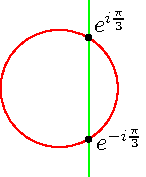
\includegraphics{./Ccp06_1.pdf}
 % Ccp06_1.pdf: 0x0 pixel, -2147483648dpi, 0.00x0.00 cm, bb=
 \caption{Exercice \ref{Ecp06}}
 \label{fig:Ccp06_1}
\end{figure}
Les nombres complexes cherchés sont donc
\begin{displaymath}
 \frac{1+i\sqrt{3}}{2}=e^{i\frac{\pi}{3}}\text{ et }\frac{1-i\sqrt{3}}{2}=e^{-i\frac{\pi}{3}}
\end{displaymath}
Voir la figure \ref{fig:Ccp06_1}.  
